\begin{itemize}
	\item При ненулевом $\delta$ распределение тёмной материи является нетермальным.
\end{itemize}
\begin{figure}[!h]
	\centering
	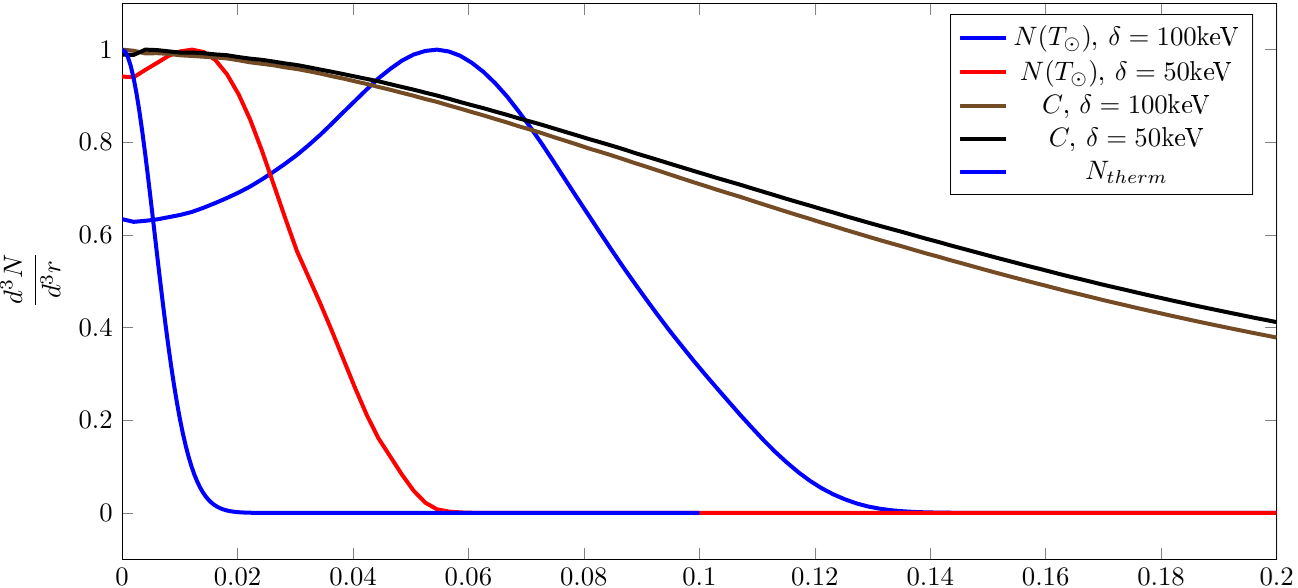
\includegraphics[width=0.8\textwidth]{images/Rdistribs.png}
	\caption{Начальное и конечное радиальное распределение частиц тёмной материи в Солнце для $m_{\chi} = 100\text{GeV}$( предполагается $\sigma_{\chi p} = 10^{-42} \text{cm}^2$, а компонента $\chi^*$ долгоживущая)}.
	\label{plot:Nrdistrib}
\end{figure}
